%%%% CAPÍTULO 1 - INTRODUÇÃO
%%
%% Deve apresentar uma visão global da pesquisa, incluindo: breve histórico, importância e justificativa da escolha do tema,
%% delimitações do assunto, formulação de hipóteses e objetivos da pesquisa e estrutura do trabalho.

%% Título e rótulo de capítulo (rótulos não devem conter caracteres especiais, acentuados ou cedilha)
\chapter{Introdução}\label{cap:introducao}

Desde o nascimento, os seres humanos desenvolvem habilidades de reconhecimento 
e identificação de objetos. Logo na primeira semana de vida, os bebês estabelecem 
rapidamente reconhecimentos individuais, discriminando e demonstrando preferência 
pela face, voz e odor de sua própria mãe \cite{vieira2017}.

O termo biometria, do grego bios (vida) e metron (medida), pode ser 
definida como ramo da ciência que estuda a identificação de aspectos físicos, biológicos e até 
comportamentais dos seres vivos. Na qual, são utilizados para distinguir indivíduos, 
a partir de suas características únicas \cite{ferreira2009}. Como, por exemplo, a face, retina, 
íris, impressões digitais, geometria da mão, etc. A biometria se tornou uma nova área de estudo 
a partir do antropologista francês Alphonse Bertillon, em 1890, quando utilizou 
conceitos de biometria para a identificação de criminosos \cite{moraes2006}. 

Dentre as tecnologias atuais de segurança, a biometria tem sido amplamente 
utilizada, seja para acessar contas bancárias, aplicativos e até controlar 
o acesso a locais públicos e privados. Atualmente, o reconhecimento facial 
é uma das biometrias mais estudadas, pois além da praticidade, é considerada uma 
das formas mais seguras de identificação \cite{zhao2003}. 

Embora a identificação facial seja uma tarefa simples para os seres humanos, 
representa um desafio considerável para os computadores. Isso se deve em 
parte às restrições impostas pelo sistema biométrico facial, que abrangem 
o controle da iluminação e dos ângulos das imagens utilizadas. Além disso, 
várias variáveis estéticas, como barba, cabelo, uso de óculos e bonés, 
problemas na lente da câmera e até mesmo a possibilidade de inserção de 
dados incorretos, podem ocasionar falhas no processo de 
reconhecimento \cite{cavalcanti2005}.

Assim, aprimorar a precisão de um sistema biométrico requer atenção 
durante o desenvolvimento, com foco na minimização de falsos 
positivos e falsos negativos no reconhecimento facial. Para superar esse 
desafio, é essencial encontrar uma abordagem que seja mais adequada ao 
sistema de autenticação por imagem. Entre as várias abordagens disponíveis, 
é fundamental avaliar a taxa de identificações incorretas e a taxa de 
casos não detectados \cite{viola2004}.

% \begin{figure}[h!]
%     \centering
%     \caption{Imagens que lembram rostos humanos}
%     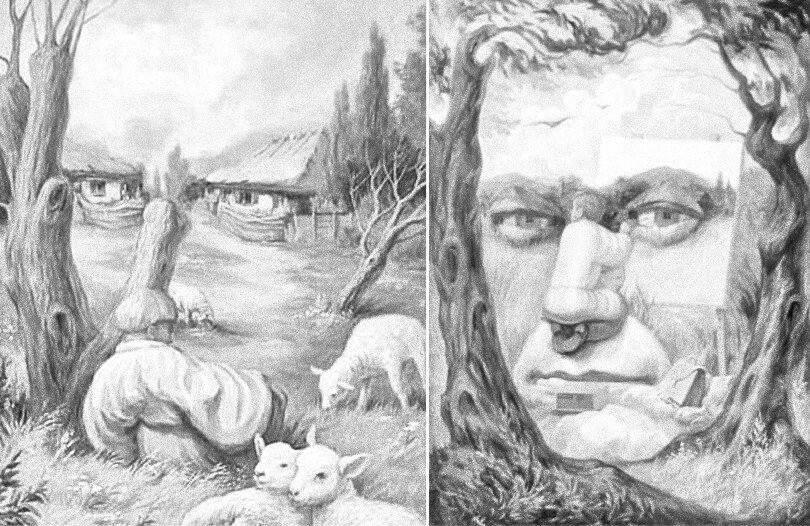
\includegraphics[scale=0.25]{figuras/pareidolia.jpg} 
%     \legend{Fonte: Adaptado de \citeonline{pareidoliaimg}.}
%     \label{fig:pareidolia}
%     \centering
% \end{figure}

Diante disso, o objetivo deste estudo é abordar o desenvolvimento de um 
protótipo que visa simplificar o controle de acesso através de um sistema 
de reconhecimento facial compacto e acessível, tornando-o de fácil 
utilização para qualquer pessoa. E também permitindo a integração 
com sistemas já existentes. 

\section{Objetivos}\label{sec:objetivos}

Nesta seção serão apresentados os objetivos deste trabalho e as etapas necessárias 
para o desenvolvimento do protótipo. Na qual, além da implementação do 
\textit{hardware}, também serão necessárias algumas etapas para a elaboração do \textit{software}, 
tendo como finalidade, obter uma alta assertividade no controle de acesso por 
reconhecimento facial.

\subsection{Objetivo geral}\label{subsec:objetivoGeral}

Este trabalho tem por objetivo realizar o estudo e desenvolvimento de um protótipo 
para controle de acesso por meio de reconhecimento facial. Para isso, 
serão utilizados algoritmos de processamento de imagens e aprendizagem 
profunda no microcontrolador ESP32-CAM.

\subsection{Objetivos específicos}\label{subsec:objetivosEspecificos}

Para que o objetivo geral seja atingido, alguma etapas essenciais deverão 
ser realizadas:

\begin{itemize}
    \item  Desenvolver o \textit{hardware} para aquisição de imagens, considerando a 
    luminosidade local e a qualidade da câmera, garantindo assim, 
    bons resultados para a etapa de reconhecimento facial;
  
    \item Implementar um código, que seja otimizado e organizado o suficiente, 
    para conseguir processar as imagens em tempo real; 
    
    \item Criar uma interface gráfica e física que permita aos usuários interagir 
    e utilizar de maneira intuitiva e simples;
    
    \item Por último, desenvolver o módulo de controle de acesso, que permitirá 
    ao administrador gerenciar e cadastrar novos usuários, concedendo ou 
    limitando o acesso conforme as necessidades.
\end{itemize}

\section{Justificativa}\label{sec:justificativa}

Os sistemas de reconhecimento facial foram uma grande solução durante a retomada 
das atividades presenciais após a pandemia do coronavírus, ajudando empresas
a promoverem uma maior segurança física, como também segurança sanitária, 
evitando contaminações e agilizando os processos. Ao contrário dos sistemas 
manuais, onde normalmente geram atrasos e demandam contato físico \cite{terra2020}.

No cotidiano, uma das formas mais comuns de garantir a segurança é por meio de 
chaves físicas, utilizadas tanto em fechaduras mecânicas quanto em fechaduras 
eletrônicas, onde essas chaves podem assumir a forma de dispositivos metálicos 
ou tags de proximidade. No entanto, apesar de sua praticidade, 
essas chaves apresentam vulnerabilidades relacionadas à possibilidade de 
fraudes, seja através de cópias não autorizadas ou do uso de técnicas como 
o ''\textit{Bump Key}'', uma ameaça frequente em diversos tipos de chaves. Um exemplo 
atual é o caso do Flipper Zero, um dispositivo projetado para clonar 
frequências de NFC, Bluetooth e RFID. De acordo com a Anatel (Agência 
Nacional de Telecomunicações), esse aparelho possui um ''potencial lesivo'' 
aos usuários, permitindo a reprodução não autorizada de controles 
remotos de portões eletrônicos, sistemas de segurança residencial, 
chaves de carro, entre outros \cite{anatel2023}. Essa capacidade de clonagem destaca 
a necessidade de abordagens mais seguras e avançadas no desenvolvimento 
de tecnologias de acesso e segurança. 

Quanto ao reconhecimento facial, um aspecto a ser considerado é a automação 
de processos. Embora a redução de custos seja um diferencial destacado 
por muitos gestores ao abordar a automação, é igualmente crucial ponderar 
sobre o potencial dessa tecnologia em proporcionar benefícios mais 
significativos para toda a cadeia produtiva. Isso implica não apenas em 
otimizar a eficiência operacional, mas também em maximizar as 
recompensas globais para os diversos setores envolvidos \cite{tiinside2023}.

Por último, destaca-se a praticidade desse sistema, uma vez que 
elimina a necessidade de memorizarem senhas ou carregarem 
chaves consigo. Esse fator tem um impacto positivo de forma geral para 
a maioria das pessoas, mas vem sendo especialmente benéfico 
para grupos de pessoas com Déficit de Atenção. 
Ao considerar que pessoas com Déficit de Atenção muitas vezes enfrentam dificuldades 
em lembrar-se de compromissos, extraviam chaves (casa ou carro) com facilidade e podem 
esquecer de tarefas cotidianas \cite{abda2023}, desta forma, sistemas de reconhecimento 
facial são soluções que favorecem e os ajudam em seu cotidiano.
